% \pgfplotsset{compat=1.15}
\usetikzlibrary{arrows}
\begin{figure}[h!]
\centering
\definecolor{ffwwzz}{rgb}{1,0.4,0.6}
\definecolor{ffqqqq}{rgb}{1,0,0}
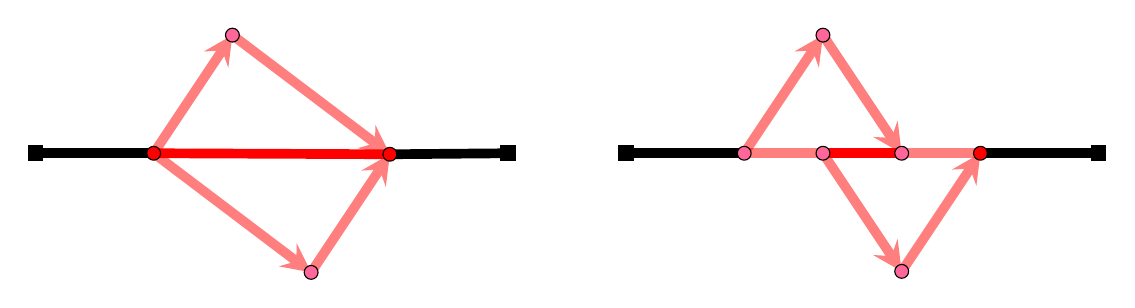
\begin{tikzpicture}[line cap=round,line join=round,>=triangle 45,x=0.5cm,y=0.5cm]
\fill[line width=2pt,fill=black] (3.8,5.2) -- (4.2,5.2) -- (4.2,4.8) -- (3.8,4.8) -- cycle;
\fill[line width=2pt,fill=black] (15.8,5.2) -- (16.2,5.2) -- (16.2,4.8) -- (15.8,4.8) -- cycle;
\fill[line width=2pt,fill=black] (18.8,5.2) -- (19.2,5.2) -- (19.2,4.8) -- (18.8,4.8) -- cycle;
\fill[line width=2pt,fill=black] (30.8,5.2) -- (31.2,5.2) -- (31.2,4.8) -- (30.8,4.8) -- cycle;
\draw [line width=3.5pt] (4,5)-- (7,5);
\begin{scope}[transparency group, opacity=0.5]
\draw [-stealth,line width=3.5pt,color=ffqqqq] (7,5) -- (9,8);
\draw [-stealth,line width=3.5pt,color=ffqqqq] (7,5) -- (11,1.974194108172913);
\draw [-stealth,line width=3.5pt,color=ffqqqq] (9,8) -- (13,4.974194108172913);
\draw [-stealth,line width=3.5pt,color=ffqqqq] (11,1.974194108172913) -- (13,4.974194108172913);
\end{scope}
\draw [line width=3.5pt,color=ffqqqq] (7,5)-- (13,4.974194108172913);
\draw [line width=3.5pt] (13,4.974194108172913)-- (16,5);
\draw [line width=3.5pt] (19,5)-- (22,5);
\draw [line width=3.5pt] (28,5)-- (31,5);
\begin{scope}[transparency group, opacity=0.5]
\draw[-stealth,line width=3.5pt, red] (22,5) -- (24,8);
\draw[-stealth,line width=3.5pt, red] (24,8) -- (26,5);
\draw[-stealth,line width=3.5pt, red] (24,5) -- (26,2);
\draw[-stealth,line width=3.5pt, red] (26,2) -- (28,5);
\end{scope}
\draw [line width=3.5pt,color=ffqqqq] (24,5)-- (26,5);
\draw [line width=3.5pt,color=ffqqqq, opacity=0.5] (22,5)-- (24,5);
\draw [line width=3.5pt,color=ffqqqq, opacity=0.5] (26,5)-- (28,5);
\begin{scriptsize}
\draw [fill=ffqqqq] (7,5) circle (2.5pt);
\draw [fill=ffwwzz] (9,8) circle (2.5pt);
\draw [fill=ffwwzz] (11,1.974194108172913) circle (2.5pt);
\draw [fill=ffqqqq] (13,4.974194108172913) circle (2.5pt);
\draw [fill=ffwwzz] (22,5) circle (2.5pt);
\draw [fill=ffqqqq] (28,5) circle (2.5pt);
\draw [fill=ffwwzz] (24,8) circle (2.5pt);
\draw [fill=ffwwzz] (26,2) circle (2.5pt);
\draw [fill=ffwwzz] (26,5) circle (2.5pt);
\draw [fill=ffwwzz] (24,5) circle (2.5pt);
\end{scriptsize}
\end{tikzpicture}
\caption{Models with complete and partial overlapping.\label{fig:2-models}}
\end{figure}